\documentclass[a4paper, body={18cm,22cm}]{article}
\usepackage{ctex}
\usepackage{amsmath}
\usepackage{forest}


\title{Homework 3: 直接构造法}
\author{李鹏达 10225101460}
\date{}

\newcommand{\fp}[1]{\operatorname{followpos}(#1)}
\newcommand{\fpp}[1]{\operatorname{firstpos}(#1)}
\newcommand{\mv}[1]{\operatorname{move}(#1)}

\begin{document}
\maketitle

\forestset{
  fp/.style={
    label=left:{\color{purple}{$\{#1\}$}}
  },
  lp/.style={
    label=right:{\color{blue}{$\{#1\}$}}
  },
}

\subsection*{1. 使用直接构造法构造这四个正则表达式的DFA,并且最小化DFA。}

\begin{enumerate}
    \item[a)] $(a | b)^*$
    
    $(a | b)^* \to (\underset{1}{a} | \underset{2}{b})^*\underset{3}{\raisebox{0.5ex}{\#}}$

    \begin{forest}
        for tree={align=center,
        s sep=20mm,             % 兄弟节点(同一层)之间的水平间距
        l sep=5mm,
        } % 设置节点格式
        [\textbullet,fp={1,2,3},lp={3}
            [*,fp={1,2},lp={1,2}
                [|,fp={1,2},lp={1,2} [$\underset{1}{a}$, fp=1, lp={1}][$\underset{2}{b}$, fp=2, lp={2}]]
            ]
            [$\underset{3}{\#}$,fp=3,lp=3]
        ]
        \node[anchor=west, align=left, text width=4cm] 
        at (current bounding box.east) [xshift=1cm] {
            {\color{purple}{purple - firstpos}} \\
            {\color{blue}{blue - lastpos}} \\
        };
    \end{forest}

    $
        \fp{1} = \{1, 2, 3\} \\
        \fp{2} = \{1, 2, 3\} \\
        \fp{3} = \{\} \\
        S_0 = \fpp{root} = \{1, 2, 3\} \\
        a: \fp{1} = \{1, 2, 3\} = S_0 \qquad \mv{S_0, a} = S_0 \\
        b: \fp{2} = \{1, 2, 3\} = S_0 \qquad \mv{S_0, b} = S_0 \\
    $

    \begin{center}
        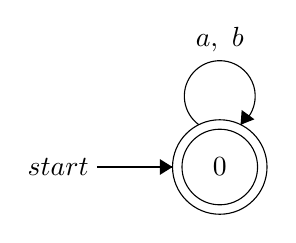
\begin{tikzpicture}[scale=0.2]
        \tikzstyle{every node}+=[inner sep=0pt]
        \draw [black] (30.5,-27.8) circle (3);
        \draw (30.5,-27.8) node {$0$};
        \draw [black] (30.5,-27.8) circle (2.4);
        \draw [black] (29.177,-25.12) arc (234:-54:2.25);
        \draw (30.5,-20.55) node [above] {$a,\mbox{ }b$};
        \fill [black] (31.82,-25.12) -- (32.7,-24.77) -- (31.89,-24.18);
        \draw [black] (22.7,-27.8) -- (27.5,-27.8);
        \draw (22.2,-27.8) node [left] {$start$};
        \fill [black] (27.5,-27.8) -- (26.7,-27.3) -- (26.7,-28.3);
        \end{tikzpicture}
        \end{center}

    显然,是最简的DFA。

    \item[b)] $(a^*|b^*)^*$
    
    $(a^*|b^*)^* \to (\underset{1}{a}^*|\underset{2}{b}^*)^*\underset{3}{\raisebox{0.5ex}{\#}}$
    
    \begin{forest}
        for tree={align=center,
        s sep=20mm,             % 兄弟节点(同一层)之间的水平间距
        l sep=5mm,
        } % 设置节点格式
        [\textbullet,fp={1,2,3},lp={3}
            [*,fp={1,2},lp={1,2}
                [|,fp={1,2},lp={1,2}
                    [*,fp=1,lp=1 [$\underset{1}{a}$, fp=1,lp=1]]
                    [*,fp=2,lp=2 [$\underset{2}{b}$, fp=2,lp=2]]
                ]
            ]
            [$\underset{3}{\#}$,fp=3,lp=3]
        ]
        \node[anchor=west, align=left, text width=4cm] 
        at (current bounding box.east) [xshift=1cm] {
            {\color{purple}{purple - firstpos}} \\
            {\color{blue}{blue - lastpos}} \\
        };
    \end{forest}

    $\fp{1}=\{1, 2, 3\} \\
    \fp{2}=\{1, 2, 3\} \\
    \fp{3}=\{\} \\
    S_0=\fpp{root}=\{1, 2, 3\} \\
    a: \fp{1}=\{1, 2, 3\} = S_0 \qquad \mv{S_0, a} = S_0 \\
    b: \fp{2}=\{1, 2, 3\} = S_0 \qquad \mv{S_0, b} = S_0 \\
    $

    \begin{center}
        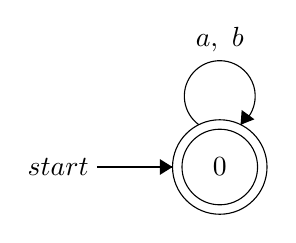
\begin{tikzpicture}[scale=0.2]
        \tikzstyle{every node}+=[inner sep=0pt]
        \draw [black] (30.5,-27.8) circle (3);
        \draw (30.5,-27.8) node {$0$};
        \draw [black] (30.5,-27.8) circle (2.4);
        \draw [black] (29.177,-25.12) arc (234:-54:2.25);
        \draw (30.5,-20.55) node [above] {$a,\mbox{ }b$};
        \fill [black] (31.82,-25.12) -- (32.7,-24.77) -- (31.89,-24.18);
        \draw [black] (22.7,-27.8) -- (27.5,-27.8);
        \draw (22.2,-27.8) node [left] {$start$};
        \fill [black] (27.5,-27.8) -- (26.7,-27.3) -- (26.7,-28.3);
        \end{tikzpicture}
        \end{center}

    显然,是最简的DFA。

    \newpage
    \item[c)] $((\varepsilon | a)b^*)^*$
    \item[] 
    $((\varepsilon | a)b^*)^* \to ((\varepsilon | \underset{1}{a})\underset{2}{b}^*)^*\underset{3}{\raisebox{0.5ex}{\#}}$

    \begin{forest}
        for tree={align=center,
        s sep=20mm,             % 兄弟节点(同一层)之间的水平间距
        l sep=5mm,
        } % 设置节点格式
        [\textbullet,fp={1,2,3},lp=3
            [*,fp={1,2},lp={1,2}
                [\textbullet,fp={1,2},lp={1,2}
                    [|,fp=1,lp=1
                        [$\varepsilon$]
                        [$\underset{1}{a}$, fp=1,lp=1]
                    ]
                    [*,fp=2,lp=2 [$\underset{2}{b}$, fp=2,lp=2]]
                ]
            ]
            [$\underset{3}{\#}$, fp=3,lp=3]
        ]
        \node[anchor=west, align=left, text width=4cm] 
        at (current bounding box.east) [xshift=1cm] {
            {\color{purple}{purple - firstpos}} \\
            {\color{blue}{blue - lastpos}} \\
        };
    \end{forest}

    $
    \fp{1}=\{1, 2, 3\} \\
    \fp{2}=\{1, 2, 3\} \\
    \fp{3}=\{\} \\
    S_0=\fpp{root}=\{1, 2, 3\} \\
    a: \fp{1}=\{1, 2, 3\} = S_0 \qquad \mv{S_0, a} = S_0 \\
    b: \fp{2}=\{1, 2, 3\} = S_0 \qquad \mv{S_0, b} = S_0 \\
    $

    \begin{center}
        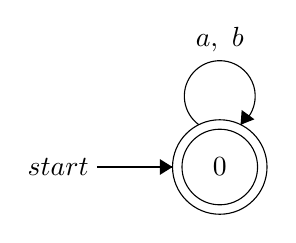
\begin{tikzpicture}[scale=0.2]
        \tikzstyle{every node}+=[inner sep=0pt]
        \draw [black] (30.5,-27.8) circle (3);
        \draw (30.5,-27.8) node {$0$};
        \draw [black] (30.5,-27.8) circle (2.4);
        \draw [black] (29.177,-25.12) arc (234:-54:2.25);
        \draw (30.5,-20.55) node [above] {$a,\mbox{ }b$};
        \fill [black] (31.82,-25.12) -- (32.7,-24.77) -- (31.89,-24.18);
        \draw [black] (22.7,-27.8) -- (27.5,-27.8);
        \draw (22.2,-27.8) node [left] {$start$};
        \fill [black] (27.5,-27.8) -- (26.7,-27.3) -- (26.7,-28.3);
        \end{tikzpicture}
        \end{center}

    显然,是最简的DFA。
    \newpage
    \item[d)] $(a|b)^*abb(a|b)^*$
    
    $(a|b)^*abb(a|b)^* \to (\underset{1}{a}|\underset{2}{b})^*\underset{3}{a}\underset{4}{b}\underset{5}{b}(\underset{6}{a}|\underset{7}{b})^*\underset{8}{\raisebox{0.5ex}{\#}}$

    \begin{forest}
        for tree={align=center,
        s sep=20mm,             % 兄弟节点(同一层)之间的水平间距
        l sep=5mm,
        } % 设置节点格式
        [\textbullet,fp={1,2,3},lp={8}
            [\textbullet,fp={1,2,3},lp={5,6,7}
                [\textbullet,fp={1,2,3},lp={5}
                    [\textbullet,fp={1,2,3},lp={4}
                        [\textbullet,fp={1,2,3},lp={3}
                            [*,fp={1,2},lp={1,2}
                                [|,fp={1,2},lp={1,2}
                                    [$\underset{1}{a}$, fp=1,lp=1]
                                    [$\underset{2}{b}$, fp=2,lp=2]
                                ]
                            ]
                            [$\underset{3}{a}$]
                        ]
                        [$\underset{4}{b}$]
                    ]
                    [$\underset{5}{b}$]
                ]
                [*,fp={6,7},lp={6,7}
                    [|,fp={6,7},lp={6,7}
                        [$\underset{6}{a}$,fp=6,lp=6] 
                        [$\underset{7}{b}$,fp=7,lp=7]
                    ]
                ]
            ]
            [$\underset{8}{\#}$,fp=8,lp=8]
        ]
        \node[anchor=west, align=left, text width=4cm] 
        at (current bounding box.east) [xshift=1cm] {
            {\color{purple}{purple - firstpos}} \\
            {\color{blue}{blue - lastpos}} \\
        };
    \end{forest}

    $
    \fp{1} = \{1,2,3\} \\
    \fp{2} = \{1,2,3\} \\
    \fp{3} = \{4\} \\
    \fp{4} = \{5\} \\
    \fp{5} = \{6,7,8\} \\
    \fp{6} = \{6,7,8\} \\
    \fp{7} = \{6,7,8\} \\
    \fp{8} = \{\} \\
    $

    $
    S_0 = \fpp{root} = \{1,2,3\} \\
    a: \fp{1} \cup \fp{3} = \{1,2,3,4\} = S_1 \qquad \mv{S_0, a} = S_1 \\
    b: \fp{2} = \{1,2,3\} = S_0 \qquad \mv{S_0, b} = S_0 \\
    \Downarrow \text{mark } S_1 \\
    a: \fp{1} \cup \fp{3} = \{1,2,3,4\} = S_1 \qquad \mv{S_1, a} = S_1 \\
    b: \fp{2} \cup \fp{4} = \{1,2,3,5\} = S_2 \qquad \mv{S_1, b} = S_2 \\
    \Downarrow \text{mark } S_2 \\
    a: \fp{1} \cup \fp{3} = \{1,2,3,4\} = S_1 \qquad \mv{S_2, a} = S_1 \\
    b: \fp{2} \cup \fp{5} = \{1,2,3,6,7,8\} = S_3 \; \mv{S_2, b} = S_3 \\
    \Downarrow \text{mark } S_3 \\
    a: \fp{1} \cup \fp{3} \cup \fp{6} = \{1,2,3,4,6,7,8\} = S_4 \qquad \mv{S_3, a} = S_4 \\
    b: \fp{2} \cup \fp{7} = \{1,2,3,6,7,8\} = S_3 \qquad \mv{S_3, b} = S_3 \\
    \Downarrow \text{mark } S_4 \\
    a: \fp{1} \cup \fp{3} \cup \fp{6} = \{1,2,3,4,6,7,8\} = S_4 \qquad \mv{S_4, a} = S_4 \\
    b: \fp{2} \cup \fp{4} \cup \fp{7} = \{1,2,3,5,6,7,8\} = S_5 \qquad \mv{S_4, b} = S_5 \\
    \Downarrow \text{mark } S_5 \\
    a: \fp{1} \cup \fp{3} \cup \fp{6} = \{1,2,3,4,6,7,8\} = S_4 \qquad \mv{S_5, a} = S_4 \\
    b: \fp{2} \cup \fp{5} \cup \fp{7} = \{1,2,3,6,7,8\} = S_3 \qquad \mv{S_5, b} = S_3 \\
    $

    \begin{table}[h]
        \centering
        \begin{tabular}{c|cc}
            & a & b \\
            \hline
            $S_0$ & $S_1$ & $S_0$ \\
            $S_1$ & $S_1$ & $S_2$\\
            $S_2$ & $S_1$ & $S_3$ \\
            $S_3$ & $S_4$ & $S_3$\\
            $S_4$ & $S_4$ & $S_5$\\
            $S_5$ & $S_4$ & $S_3$\\
        \end{tabular}
    \end{table}

    \begin{center}
        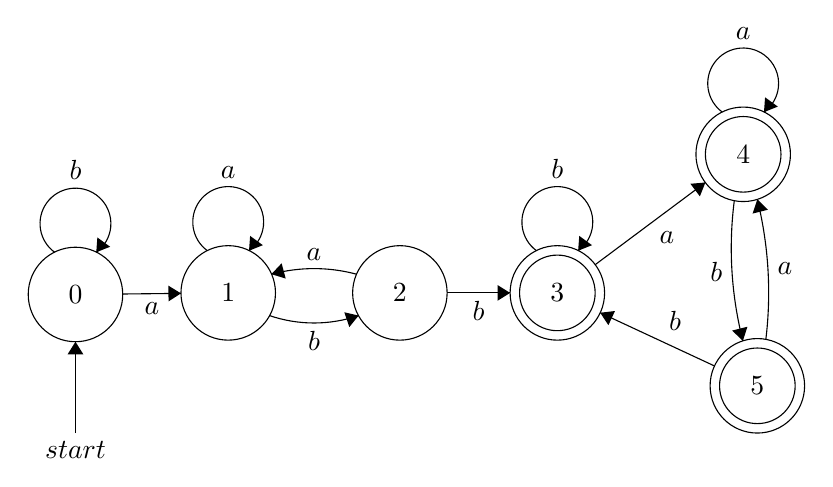
\begin{tikzpicture}[scale=0.2]
        \tikzstyle{every node}+=[inner sep=0pt]
        \draw [black] (9.7,-28.2) circle (3);
        \draw (9.7,-28.2) node {$0$};
        \draw [black] (19.4,-28.1) circle (3);
        \draw (19.4,-28.1) node {$1$};
        \draw [black] (30.3,-28.1) circle (3);
        \draw (30.3,-28.1) node {$2$};
        \draw [black] (40.3,-28.1) circle (3);
        \draw (40.3,-28.1) node {$3$};
        \draw [black] (40.3,-28.1) circle (2.4);
        \draw [black] (52.1,-19.3) circle (3);
        \draw (52.1,-19.3) node {$4$};
        \draw [black] (52.1,-19.3) circle (2.4);
        \draw [black] (53,-34) circle (3);
        \draw (53,-34) node {$5$};
        \draw [black] (53,-34) circle (2.4);
        \draw [black] (12.7,-28.17) -- (16.4,-28.13);
        \fill [black] (16.4,-28.13) -- (15.6,-27.64) -- (15.61,-28.64);
        \draw (14.55,-28.66) node [below] {$a$};
        \draw [black] (8.377,-25.52) arc (234:-54:2.25);
        \draw (9.7,-20.95) node [above] {$b$};
        \fill [black] (11.02,-25.52) -- (11.9,-25.17) -- (11.09,-24.58);
        \draw [black] (18.077,-25.42) arc (234:-54:2.25);
        \draw (19.4,-20.85) node [above] {$a$};
        \fill [black] (20.72,-25.42) -- (21.6,-25.07) -- (20.79,-24.48);
        \draw [black] (27.684,-29.538) arc (-71.04396:-108.95604:8.725);
        \fill [black] (27.68,-29.54) -- (26.77,-29.33) -- (27.09,-30.27);
        \draw (24.85,-30.51) node [below] {$b$};
        \draw [black] (22.145,-26.915) arc (105.08761:74.91239:10.394);
        \fill [black] (22.14,-26.91) -- (23.05,-27.19) -- (22.79,-26.22);
        \draw (24.85,-26.06) node [above] {$a$};
        \draw [black] (33.3,-28.1) -- (37.3,-28.1);
        \fill [black] (37.3,-28.1) -- (36.5,-27.6) -- (36.5,-28.6);
        \draw (35.3,-28.6) node [below] {$b$};
        \draw [black] (42.7,-26.31) -- (49.7,-21.09);
        \fill [black] (49.7,-21.09) -- (48.75,-21.17) -- (49.35,-21.97);
        \draw (47.26,-24.2) node [below] {$a$};
        \draw [black] (38.977,-25.42) arc (234:-54:2.25);
        \draw (40.3,-20.85) node [above] {$b$};
        \fill [black] (41.62,-25.42) -- (42.5,-25.07) -- (41.69,-24.48);
        \draw [black] (50.777,-16.62) arc (234:-54:2.25);
        \draw (52.1,-12.05) node [above] {$a$};
        \fill [black] (53.42,-16.62) -- (54.3,-16.27) -- (53.49,-15.68);
        \draw [black] (52.08,-31.147) arc (-165.72202:-187.27092:23.856);
        \fill [black] (52.08,-31.15) -- (52.37,-30.25) -- (51.4,-30.49);
        \draw (50.8,-26.75) node [left] {$b$};
        \draw [black] (52.996,-22.161) arc (13.90536:-6.89829:24.665);
        \fill [black] (53,-22.16) -- (52.7,-23.06) -- (53.67,-22.82);
        \draw (54.26,-26.55) node [right] {$a$};
        \draw [black] (50.28,-32.74) -- (43.02,-29.36);
        \fill [black] (43.02,-29.36) -- (43.54,-30.15) -- (43.96,-29.25);
        \draw (47.77,-30.54) node [above] {$b$};
        \draw [black] (9.7,-37) -- (9.7,-31.2);
        \draw (9.7,-37.5) node [below] {$start$};
        \fill [black] (9.7,-31.2) -- (9.2,-32) -- (10.2,-32);
        \end{tikzpicture}
        \end{center}

        $G_1 = \{3,4,5\} \\
        G_2 = \{0,1,2\} \\
        $

        \begin{table}[h]
            \begin{tabular}{cc}
                $a$ & $b$ \\
                \hline
                $3 \to 4$ & $3 \to 3$ \\
                $4 \to 4$ & $4 \to 5$ \\
                $5 \to 4$ & $5 \to 3$ \\
            \end{tabular}
        \end{table}

        所以 $G_1$ 是不可分的。

        \begin{table}[h]
            \begin{tabular}{cc}
                $a$ & $b$ \\
                \hline
                $0 \to 1$ & $0 \to 0$ \\
                $1 \to 1$ & $1 \to 2$ \\
                $2 \to 1$ & $2 \to 3$ \\
            \end{tabular}
        \end{table}

        所以 $G_2$ 可以分成 $\{0\}$, $\{1\}$, $\{2\}$。


        化简后的DFA如下:

        \begin{center}
            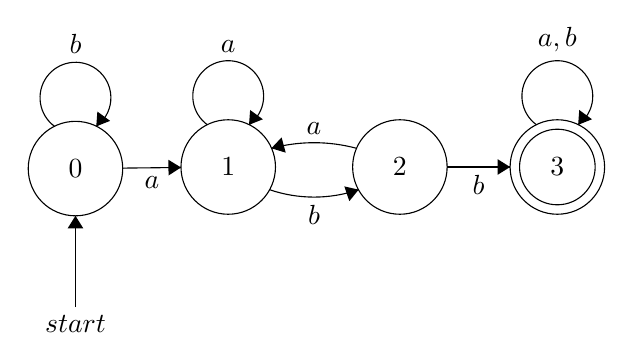
\begin{tikzpicture}[scale=0.2]
            \tikzstyle{every node}+=[inner sep=0pt]
            \draw [black] (9.7,-28.2) circle (3);
            \draw (9.7,-28.2) node {$0$};
            \draw [black] (19.4,-28.1) circle (3);
            \draw (19.4,-28.1) node {$1$};
            \draw [black] (30.3,-28.1) circle (3);
            \draw (30.3,-28.1) node {$2$};
            \draw [black] (40.3,-28.1) circle (3);
            \draw (40.3,-28.1) node {$3$};
            \draw [black] (40.3,-28.1) circle (2.4);
            \draw [black] (12.7,-28.17) -- (16.4,-28.13);
            \fill [black] (16.4,-28.13) -- (15.6,-27.64) -- (15.61,-28.64);
            \draw (14.55,-28.66) node [below] {$a$};
            \draw [black] (8.377,-25.52) arc (234:-54:2.25);
            \draw (9.7,-20.95) node [above] {$b$};
            \fill [black] (11.02,-25.52) -- (11.9,-25.17) -- (11.09,-24.58);
            \draw [black] (18.077,-25.42) arc (234:-54:2.25);
            \draw (19.4,-20.85) node [above] {$a$};
            \fill [black] (20.72,-25.42) -- (21.6,-25.07) -- (20.79,-24.48);
            \draw [black] (27.684,-29.538) arc (-71.04396:-108.95604:8.725);
            \fill [black] (27.68,-29.54) -- (26.77,-29.33) -- (27.09,-30.27);
            \draw (24.85,-30.51) node [below] {$b$};
            \draw [black] (22.145,-26.915) arc (105.08761:74.91239:10.394);
            \fill [black] (22.14,-26.91) -- (23.05,-27.19) -- (22.79,-26.22);
            \draw (24.85,-26.06) node [above] {$a$};
            \draw [black] (33.3,-28.1) -- (37.3,-28.1);
            \fill [black] (37.3,-28.1) -- (36.5,-27.6) -- (36.5,-28.6);
            \draw (35.3,-28.6) node [below] {$b$};
            \draw [black] (38.977,-25.42) arc (234:-54:2.25);
            \draw (40.3,-20.85) node [above] {$a,b$};
            \fill [black] (41.62,-25.42) -- (42.5,-25.07) -- (41.69,-24.48);
            \draw [black] (9.7,-37) -- (9.7,-31.2);
            \draw (9.7,-37.5) node [below] {$start$};
            \fill [black] (9.7,-31.2) -- (9.2,-32) -- (10.2,-32);
            \end{tikzpicture}
            \end{center}

\end{enumerate}

\end{document}
